\documentclass[11pt]{article}
\usepackage{fullpage}
\usepackage{fontspec}
\setmainfont{Times New Roman}
\usepackage{graphicx,capt-of,amsmath,float,indentfirst,xcolor,listings}
\begin{document}

\title{Final Report}
\author{Weijun Huang, Lihaomin Qiu, Molan Yang, Yifan Jiang}

\maketitle

\section{assembler}

In the assembler, our objective is to translate the corresponding assembly code into binary format. The instructions in the assembler are the same as in the emulator, covering a range of operations from arithmetic operations to branching, single data transfer, and special instructions.

\subsection{structure}

Similar to the emulator, our assembler project follows a specific file and directory structure.  The main file, "assemble.c," is located outside of any directories. Inside the main directory, we have a directory for each type of instruction, including arithmetic operations, branching, single data transfer, and special instructions. Additionally, we have an additional subdirectory named "parser" that contains the files related to input handling and parsing. Furthermore, certain crucial files like "Util", "parseformat," and "symboltable" are located directly within the "assembles" directory to prevent cyclic includes. By doing so, efficient referencing of these files can be ensured throughout the project, as they are extensively utilized by various other components.

Furthermore, To streamline the build process, we have implemented a makefile in each directory. The makefile in the outer directory takes care of calling the corresponding makefile in the inner directory, resulting in the generation of library files. This approach simplifies the inclusion of necessary files and ensures proper linkage between different components of the assember.

By following this structured approach, we promote modularity, maintainability, and ease of development. It allows us to work on specific instruction types independently while ensuring smooth integration and collaboration among different components.

\subsection{implementation}
In the main function of the assembler, two arguments are received: the input and output files. The first pass of the assembler involves building a symbol table, implemented using a dynamic array. It reads each line and identifies the lines that use labels, adding the label name and its corresponding address to the symbol table.

After the first pass, the second pass begins. This pass reads each line, removes redundant white spaces, and uses the parser to determine the type of instruction by checking the opcode. If an alias instruction is encountered, it is renamed using a separate function. The parser then parses the remaining line into different elements by using the comma as a delimiter. These elements, along with the opcode, are passed to the corresponding tokenizer, which converts them into binary code.  The resulting binary code is stored as an $uint32\_t$ since it represents a 32-bit binary value. Finally, the binary code is written into a binary file as output.

\subsection{debugging}
The debugging process in the assembler was challenging but relatively easier compared to the emulator, as each line has less direct relation to other lines.

One significant issue we encountered was dealing with white spaces. During the debugging process, we encountered test cases that occasionally included unnecessary spaces at the start, end, or after commas. Moreover, it was crucial to ensure the presence of specific spaces between the opcode and the remaining line, as well as within shift statements. The challenge in this scenario was identifying the commas that needed to be removed while preserving the structural integrity of the code.

Another challenge arose when checking and converting strings into decimal or hexadecimal values, as they either start with or without '\#' symbol. We also faced problems while handling aliases, as new memory needed to be allocated and a pointer returned after the alias was generated to pass it into the tokeniser function. Furthermore, we experienced difficulties when running the testsuite on macOS devices. However, we were able to resolve this issue by utilizing lab machines for testing purposes.

\section{turn on LED on a Raspberry Pi}
In the implementation of Part 3, our group adopted a systematic approach, partitioning the task into distinct phases. Initially, our objective was to compose the assembler code, enabling the illumination of the LED. Contrary to expectations, this proved rather arduous due to the intricacies involved in passing immediate values to registers. Our preliminary efforts did not yield a solution, compelling us to utilise labels for the immediate values, which diverged from our original plan.

Subsequently, our endeavour was to effectuate the LED to illuminate for a brief interval and subsequently deactivate. This ostensibly rudimentary task was fraught with unexpected complexities. The wait function did not exhibit the anticipated performance, likely attributable to an excessive utilisation of registers. Additionally, we inadvertently neglected the necessity to replenish the buffer with each iteration of LED activation, which inadvertently extended the duration of execution. Nevertheless, through persistent efforts, we succeeded in effectuating the LED to blink quintuple times. It is noteworthy that one of our group members displayed proficiency in comprehending the read function and status verification function, which notably expedited our progress. Conclusively, we refined our codebase and achieved completion of Part 3.

\subsection{Challenges}
Although the overarching architecture of the program in Part 3 was ostensibly simplistic, the utilisation of an A64 instruction subset, which was supported by the emulator and assembler developed in the first and second parts of our project, considerably circumscribed our latitude during implementation. Certain instructions, including ‘mov’, were either inexistent or encumbered with constraints within this subset, necessitating the formulation of innovative and elaborate solutions. \\

Furthermore, debugging presented formidable challenges. The emulator, albeit beneficial, entailed a protracted implementation phase. Consequently, when it was ultimately constructed by one of our group members, we were nearing the culmination of the project. The impediments in the program were enigmatic, and deciphering the causal factors, particularly pertaining to the 'wait' function, was taxing. Although the program was concise, it did not fulfill its designated purpose. As a corrective measure, we adopted more oblique debugging methodologies, encompassing strategies such as eliminating potential problematic segments of the program, modulating values in pivotal registers (e.g., registers retaining the LED status), and repositioning sections of the program to the forefront to ascertain proper execution. This multifaceted approach proved instrumental in surmounting the challenges, encompassing the issues with the 'wait' function.

\section{extension: Super fabulous piano simulator}

\begin{figure}[H]
	\centering
	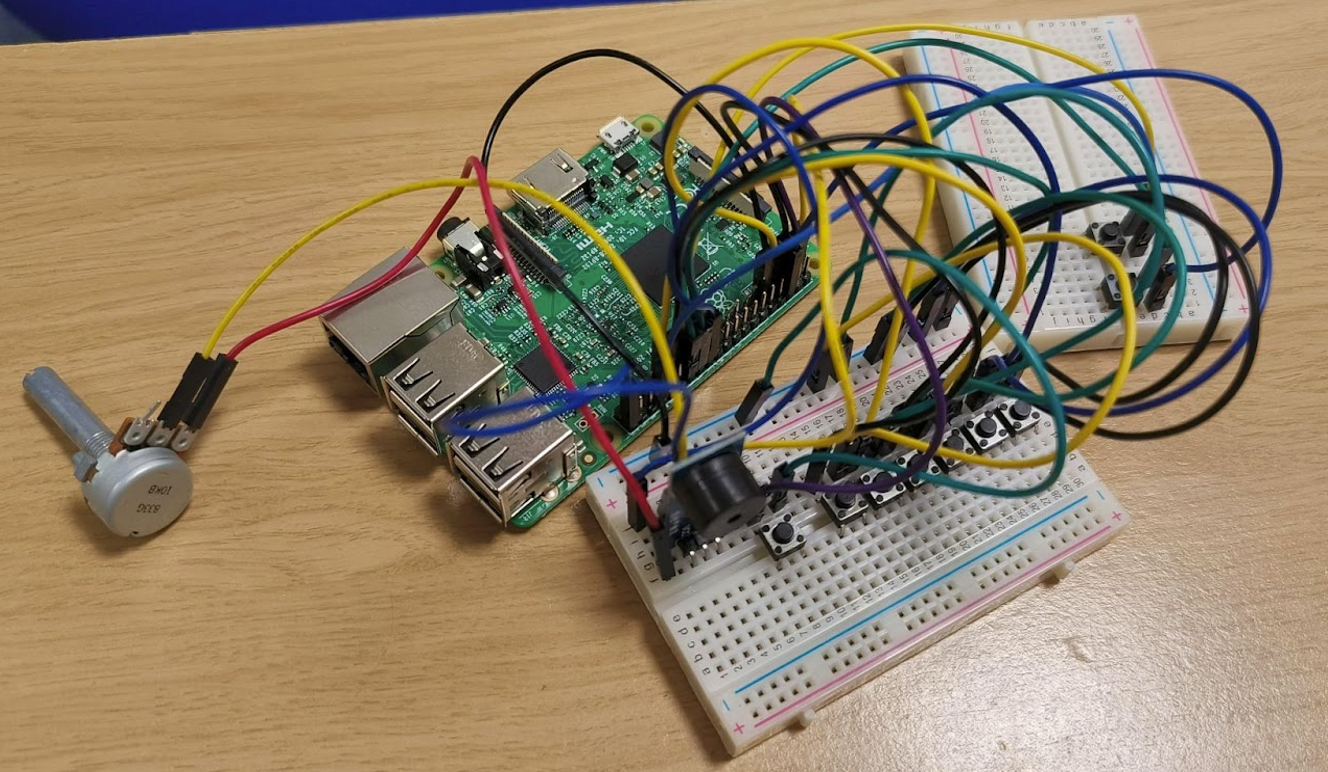
\includegraphics[width=10cm]{src/extension.png}
	\caption{A physical connection for raspberry pi}
	\label{fig:extension}
\end{figure}


Our super fabulous piano simulator can not only simulate C major notes, but also allows users to switch octaves by pressing specific buttons. What’s even better is that the volume of the speaker(buzzer) can be adjusted precisely when you rotate the potentiometer, which effectively avoids bothering others.
We are sure that this “piano” will give you a great experience and that your musical career will start here!

\subsection{challenges}

To be honest, designing and constructing the simulator is quite a big challenge to all four of us since we do not have any relevant lectures in year 1. 
In the stage of design, we met such 3 challenges:
Firstly, we do not understand what we can do with this raspberry 3b+ microcontroller, unfamiliar with all the GPIO ports and struggling to install an OS for it. What’s more, we do not know what kinds of electronic components we need to use and how to get some of the components which are not provided in the box. The last challenge is that we only have one Raspberry but part 3 and extension both need it so it is hard to do parallelism.

Fortunately, we manage to overcome all three challenges:
For the first challenge, we searched for some guidance on how to install the OS on a Raspberry 3B+ and read the official documentation to get a thorough understanding of the microcontroller. By researching similar projects(most of them are built by using an Arduino uno), we find out which electronic components are useful and thus we pass the second challenge. The last one is hard to overcome since it is not necessary enough for us to buy a second microcontroller, so we carefully share out the work and cooperate with one another.

In the stage of construction we met so many difficulties that I can not write down all of them here. So I chose three of them to talk about.

The biggest one and the one which makes us waste three hours is that some of the GPIO ports on the microcontroller can not be used for our button(since we need to connect so many buttons to implement the simulator) or maybe some of the ports are broken on our Raspberry. We were confused when we tried to detect if a button is pressed or not, but sometimes it does not work. Another key challenge is that we do not know how to let our buzzer buzz at a specific frequency, we tried to use PWM frequency in our library but the function does not work. The third one but also an important one is that we tried to find some information or tutorial on how to connect raspberry to these components but the sources are quite few and most of them are written in python instead of C.

The same, we properly solve all these problems. Fortunately, the first challenge was solved by some kind of coincidence. By trying to replace the wire/button thousands of times but find it is useless, tried to analyse it from the program level but also found nothing. Just when we were about to give up, we surprisingly found the GPIO 0 and GPIO 1 to be very reliable. So we connected the switching button to these two ports. The second challenge is so tricky that we changed our mind so that instead of focusing on the functions that are provided by the library, we tried to make it possible “physically”. Fortunately, we found a useful way to make it work. We first divide the specific period by two and first set the buzz on and after half period, set the buzzer off and sleep for another half period. As a result, the buzzer can buzz at the specific frequency and thus we could get the notes we want. The third problem is quite confusing and tough since we cannot build a library from scratch by ourselves. At the beginning, we found a useful library which is called $Wiring_Pi$. However, when we typed $Wiring\_Pi.h$ in our IDE, it was underlined by red because the library is not supported now. We were so disappointed at that moment. The appearance of one library called “pigpio” saves us from hell. Although the information about this library is quite limited, it is still better than nothing. After a period of research, we finally implemented the functions by using this library. 


\subsection{testing}

Briefly speaking we experience three stages of testing:

When we finished the first octave and did not implement the volume adjustment system, what we needed to test was just the seven buttons and the buzzer. In the beginning, we mistook the frequencies of some notes. It sounded weird when we played it, so we quickly knew where the problem was and solved it. Just after that, we added the potentiometer to adjust the volume(because when we tested stage 1 in the lab, it seemed that it made so much noise that someone else came to remind us to keep the voice down) and everything went well. Several hours later, we tried to add the octave adjustment function, but we encountered unprecedented difficulties as talked above. Fortunately, we solved the problem after three hours of foolish attempts and got the final version. 

\section{reflection}

\subsection{group reflection}
As a group, reflecting upon the completion of our C project, we acknowledge both our accomplishments and areas where we could have performed better.

One of the key elements that significantly contributed to our efficiency was our preference to collaborate in person. The immediate exchange of ideas and real-time problem-solving greatly aided the progress of our project. Given the advantages that we reaped from this approach, we are unanimous in our decision to continue employing this strategy in our future endeavours.

However, we identified that our method of dividing the workload, which was mainly based on following the specification, led to an uneven distribution. Some members ended up with a substantially larger workload. In hindsight, a more balanced approach would have been to assess the entire project first and then allocate the tasks, ensuring a fairer share of responsibilities. This is something we will strive to implement next time.

Another area that necessitated attention was the variance in coding styles among team members. This discrepancy made our codebase less cohesive and somewhat challenging to read. We collectively realise the importance of standardising our coding conventions. Before commencing any future project, we will establish a formal coding style to ensure consistency throughout the codebase.

In addition to the aforementioned reflections, we also recognized an issue related to hardware utilisation during the development of the third section and the extension part of the project. As these sections necessitated testing on the Raspberry Pi, we often found ourselves frequently exchanging the device amongst team members. This not only led to inefficiencies but also made the development process cumbersome for those who needed access to the hardware at the same time.

To mitigate this issue in the future, we will need to strategically plan and allocate project timelines. By doing this, we can ensure that no two segments of the project that require access to the same hardware are being worked on simultaneously. This will reduce the need for frequent hardware swaps and make the workflow smoother and more efficient for all team members.

Furthermore, we identified the critical importance of timely communication with our mentor. Engaging in regular dialogue and actively seeking guidance can facilitate better understanding and quicker resolution of challenges. In future projects, we commit to fostering an open channel of communication with our mentor, enabling us to glean insights, receive feedback, and make informed decisions.

In conclusion, our group learned valuable lessons from the C project. We plan to apply these lessons, including better workload allocation, standardisation of coding styles, strategic hardware utilisation planning, and proactive communication with our mentor, to improve our collaboration and project execution in the future.



\subsection{individual reflections}
\subsubsection{Weijun huang}
Throughout the project, as a team leader, I made efforts to guide my group mates in separating tasks effectively. However, the problem arose when the tasks were unevenly distributed, as I based the separation on specifications rather than estimated time. This resulted in some group mates having to assist with debugging, which was quite frustrating. Additionally, working on the project as a team taught me valuable lessons on collaboration and the significance of setting deadlines to allocate equal time to each task, ensuring that we didn't end up with all the work left until the last week. 

Furthermore, my coding skills were significantly enhanced during the project, particularly in the area of string parsing for the assembler. I also learned the importance of maintaining a well-organised code and file structure. However, there are areas for improvement. For instance, I realised the importance of understanding the work my teammates were doing, even if it was not directly related to my assigned tasks (especially since I was not involved in part 3, so I was unsure about their progress). Additionally, while working on extensions, although I managed to solve some problems through trial and error, I lacked a thorough understanding of the underlying reasons. Moving forward, I believe it would be beneficial for me to strive for a deeper understanding of the reasons behind the issues I encounter.

\subsubsection{Lihaomin Qiu}
In part1 and part2, I was responsible for Single Data Transfer. It seemed that I always finished the code very fast and easily passed all the generated tests and started to write the report. However, when it came to the general test, I could also always find some small mistakes which result in some errors in general tests. This taught me that when I write codes in the future, I should never be complacent and should always check my codes carefully even if they can pass all the basic tests.

In the extension part, I mainly focused on the hardware part but since I have never used a Raspberry Pi  microcontroller before(I used Arduino and 51 before) so I made some mistakes when choosing the port to connect the buttons which led to wasting 3 hours of precious time. Other than this error, I also made a mistake when using the potentiometer. I forgot how the potentiometer is composed, thus I bought useless ADCs chips(Analogy to digital converter) and delayed the start time of our extension. Based on this, I decided to learn more about electronic components this summer and be more careful when making such decisions next time.

\subsubsection{Molan Yang}
Throughout the project, our group divided the work efficiently, and my role was to design the interface that linked my part of the work with other parts of the project. In Part 1 and Part 2, my responsibility was data processing. However, I faced challenges in Part 1 as I was not very familiar with the C language, resulting in several mistakes. These mistakes caused issues within the team, especially because most test cases relied on data processing instructions. Furthermore, the comments I wrote were not clear to my teammates, leading to confusion. However, I took the feedback from the first mentor meeting seriously and worked on improving these weaknesses. In Part 2, I made fewer mistakes and resolved bugs more quickly compared to Part 1. I ensured to leave useful comments next to my code and identified potential problems in others' programs. In Part 3 and 4, my main focus was on Part 3. By that time, our team had developed better cooperation and efficient communication. Despite Part 3 being more challenging than expected, we managed to finish it faster than most other groups, mainly because we decided to work in person, which proved to be more efficient than remote collaboration.

\subsubsection{Yifan Jiang}
In a recent academic project, I took on the key role of working on parts one and two, focusing on branch and special instructions, and also handled assembly code in the third part. Our team maintained good relationships among members. Despite some disagreements, we kept a peaceful and open atmosphere which allowed for honest communication. This made it easier to solve differences and greatly improved our project. While working on the project, I noticed I was good at refining the report. Paying attention to details and clearly explaining our findings significantly improved our document. I felt proud seeing these skills in action.

On the flip side, this project revealed some weaknesses in my skills. I struggled with fixing errors in the code and found traditional debugging methods to be inefficient. Also, my scripting skills needed improvement, which would have helped automate repetitive tasks and eased our workload. Reflecting on this experience, in future projects with a diverse team, I would focus on improving my debugging skills and learning scripting languages for efficiency. I would also encourage an environment that supports open communication and teamwork. Overall, this project has been a learning journey, helping me understand my strengths and areas for improvement. Recognizing the importance of teamwork and communication is invaluable, and I will work on my weaknesses and leverage my strengths in future academic collaborations.
\end{document}
